\documentclass{article}
\usepackage{xcolor}
\usepackage{graphicx}
\usepackage{microtype}
\usepackage{amsmath}
\usepackage{hanging}
\usepackage[paperwidth=24in,paperheight=30in,top=1in,bottom=2in,left=1in,right=1in]{geometry}
\usepackage{fontspec}
\pagestyle{empty}
% DIN 1451 Std or DIN 30640 Std for descriptions
% Trade Gothic LT for titles
\begin{document}
\begin{minipage}[c]{20in}
{ 
\fontspec{Trade Gothic LT}[Color=red]
\fontsize{3in}{0.5in}\selectfont 
\bfseries
% SOMETHING FOR 

% \vspace{0.5in}

% EVERYONE:

% \vspace{0.5in}

% A COMEDY TONIGHT?

ROUND UP THE
}
{ 
\fontspec{Trade Gothic LT}[Color=red]
\fontsize{3.97in}{0.5in}\selectfont 
\bfseries
% \vspace{0.5in}

{\addfontfeature{Color=darkgray} (UN)}USUAL 

\vspace{0.4in}

SUSPECTS!
}
\end{minipage}
\vspace{1in}\\
\colorbox{white}{
\begin{minipage}{21in}
\centering
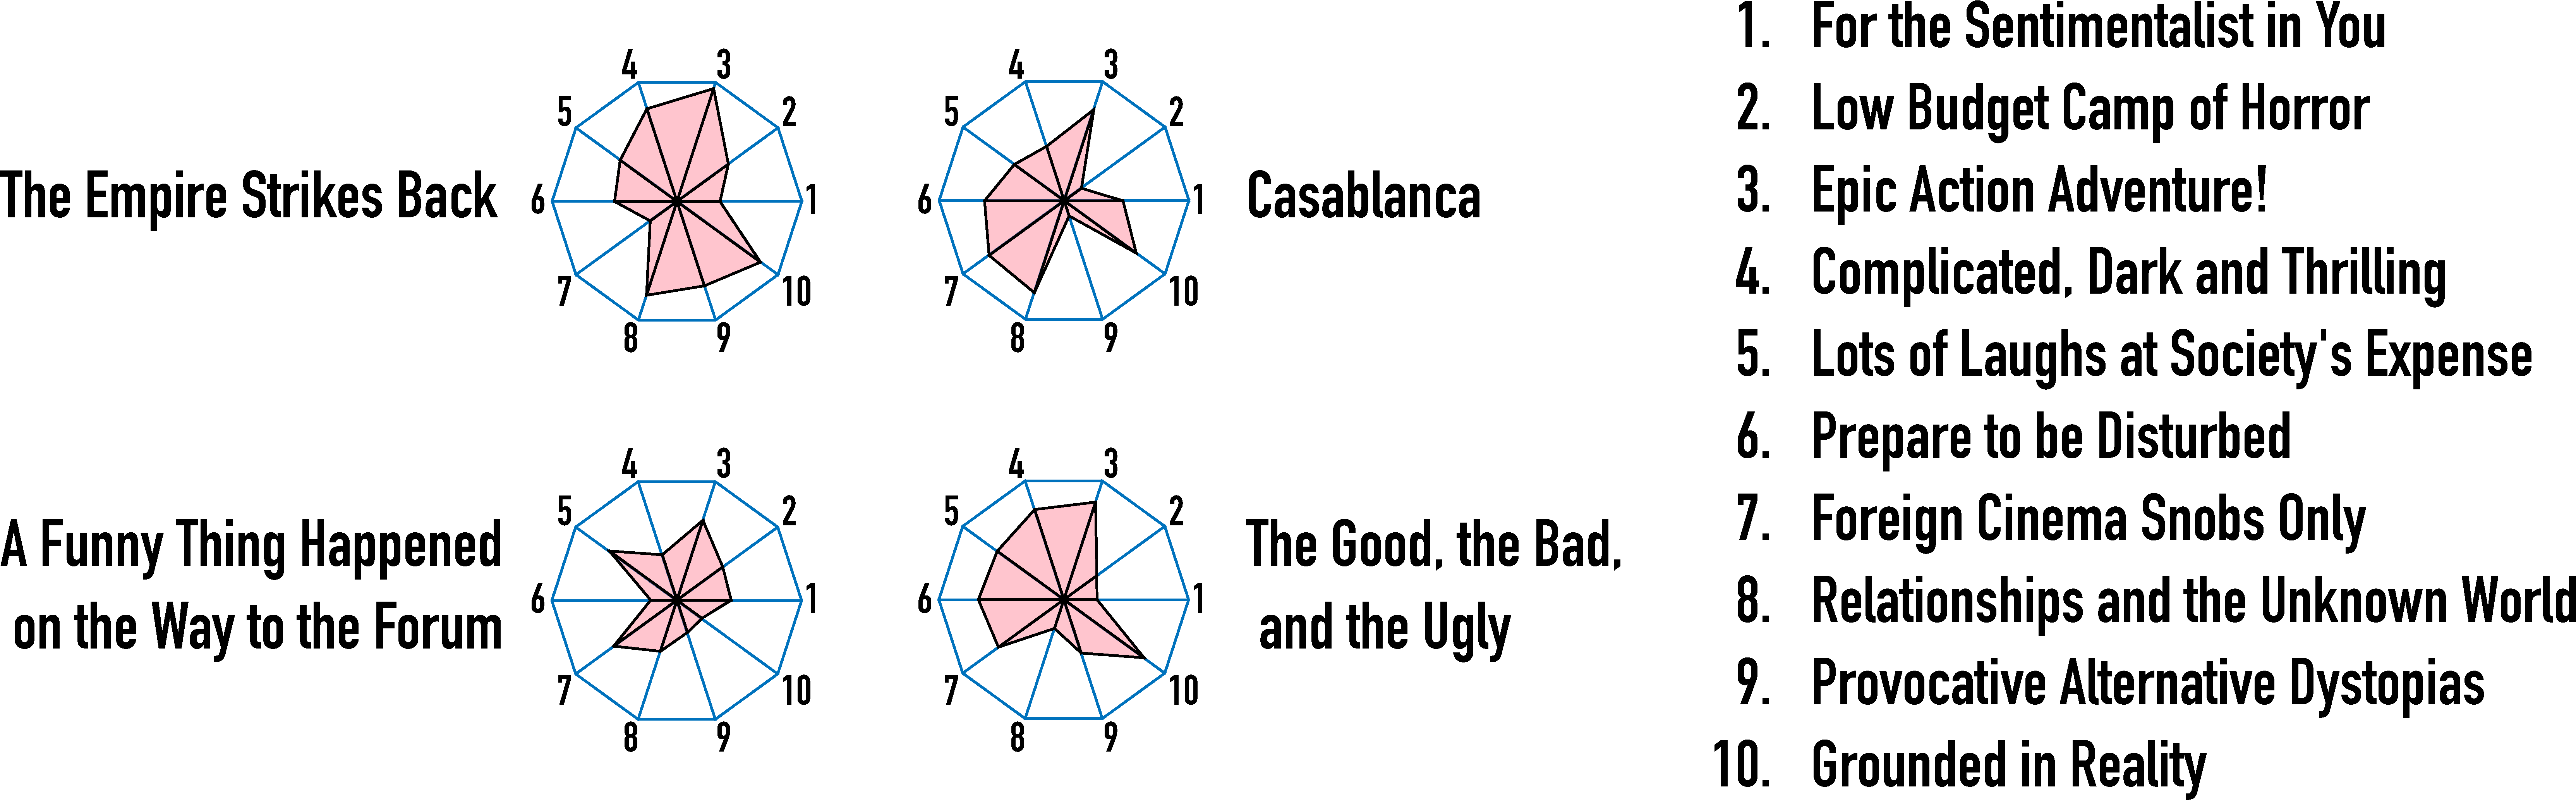
\includegraphics[width=21in]{figure.pdf}
\end{minipage}
}
\vspace{1in}\\
{
\fontspec{DIN 1451 Std}[Color=black]
\fontsize{1in}{1em}\selectfont 
CHRIS CURRO
}
{
\fontspec{DIN 1451 Std}[Color=black]
\fontsize{0.8in}{1em}\selectfont 
EE '15,
}
{
\fontspec{DIN 1451 Std}[Color=black]
\fontsize{1in}{1em}\selectfont 
DAVID KATZ
}
{
\fontspec{DIN 1451 Std}[Color=black]
\fontsize{0.8in}{1em}\selectfont 
EE '15 AND
}
{
\fontspec{DIN 1451 Std}[Color=black]
\fontsize{1in}{1em}\selectfont 
HARRISON ZHAO
}
{
\fontspec{DIN 1451 Std}[Color=black]
\fontsize{0.8in}{1em}\selectfont 
EE '16
}

\vspace{0.2in}

{
\fontspec{DIN 1451 Std}[Color=black]
\fontsize{0.8in}{1em}\selectfont 
\noindent ADVISOR: SAM KEENE
}
\vspace{0.8in}\\
\begin{minipage}{11in}
{
	\fontspec{DIN 1451 Std}[Color=black,Ligatures=TeX]
	\fontsize{0.58in}{6em}\selectfont

	We created a movie recommendation system that allows users to pick what
	they're interested in based on ten features, and how important it is that we
	pick movies similar to each of those features. The specific features were
	learned by a statistical model called an autoencoder which found
	meaningful relationships between a set of one thousand tags on each movie
	to create a set of ten descriptors. Some of the feature ratings produced by
	our autoencoder can be seen above.

	% \vspace{0.5in}
	% \begin{hangpunct}
	% In our interactive demo, a user can load a given movie's set of features by typing 
	% its name into the search bar at the top of the page and then clicking
	% ``Load Features.'' The user can then adjust feature values and relevancies to fit
	% their particular tastes. The user then clicks ``Recommend Movies'' and enjoys 
	% our suggestions!
	% \end{hangpunct}

}
\end{minipage} 
\hfill
\begin{minipage}{8in}
{
	\fontspec{DIN 1451 Std}[Color=black]
	\fontsize{0.55in}{5.5em}\selectfont
	\begin{tabbing}
	Source Code: \= github.com/katzdave/MovieRecommendation\\
	More Info: \> ee.cooper.edu/\textasciitilde{}curro/movieRec.pdf\\
	Note: \> An interactive demo will be available for \\ \> the duration of the public exhibition.
	\end{tabbing}
}
\end{minipage} 
\end{document}

